\documentclass[10pt]{beamer}
\usepackage[utf8]{inputenc}

\usepackage{graphicx}
\usepackage{minted}     % syntax highlighting
\usepackage{listings}

\newcommand{\code}[1]{\texttt{#1}}

\usetheme{Madrid}
%\usetheme{boxes}
%\usetheme{Singapore}
%\usetheme{Pittsburgh}

\usecolortheme{whale}
%\usecolortheme{dove}
%\usecolortheme{lily}
\usecolortheme{orchid}

\title{An educational kernel for the Raspberry Pi}
\subtitle{CS310 - Presentation}
\author{Thomas Archbold}
\date{\today}

\begin{document}

\begin{frame}
    \titlepage
\end{frame}

\begin{frame}{Introduction}

\begin{columns}[c]
    \column{.5\textwidth}
    Operating systems are some of the most pervasive pieces of software around, but also some of the most complex \\~\\

    The introduction of the Raspberry Pi has made computers much more accessible - allows and encourages experimenting at all levels \\~\\

    There are several official operating systems for the Pi - NOOBS, Raspbian, Windows IoT core, PiNET - but none provide a resource to learn about the operating system itself

    \column{.5\textwidth}
    \begin{figure}
        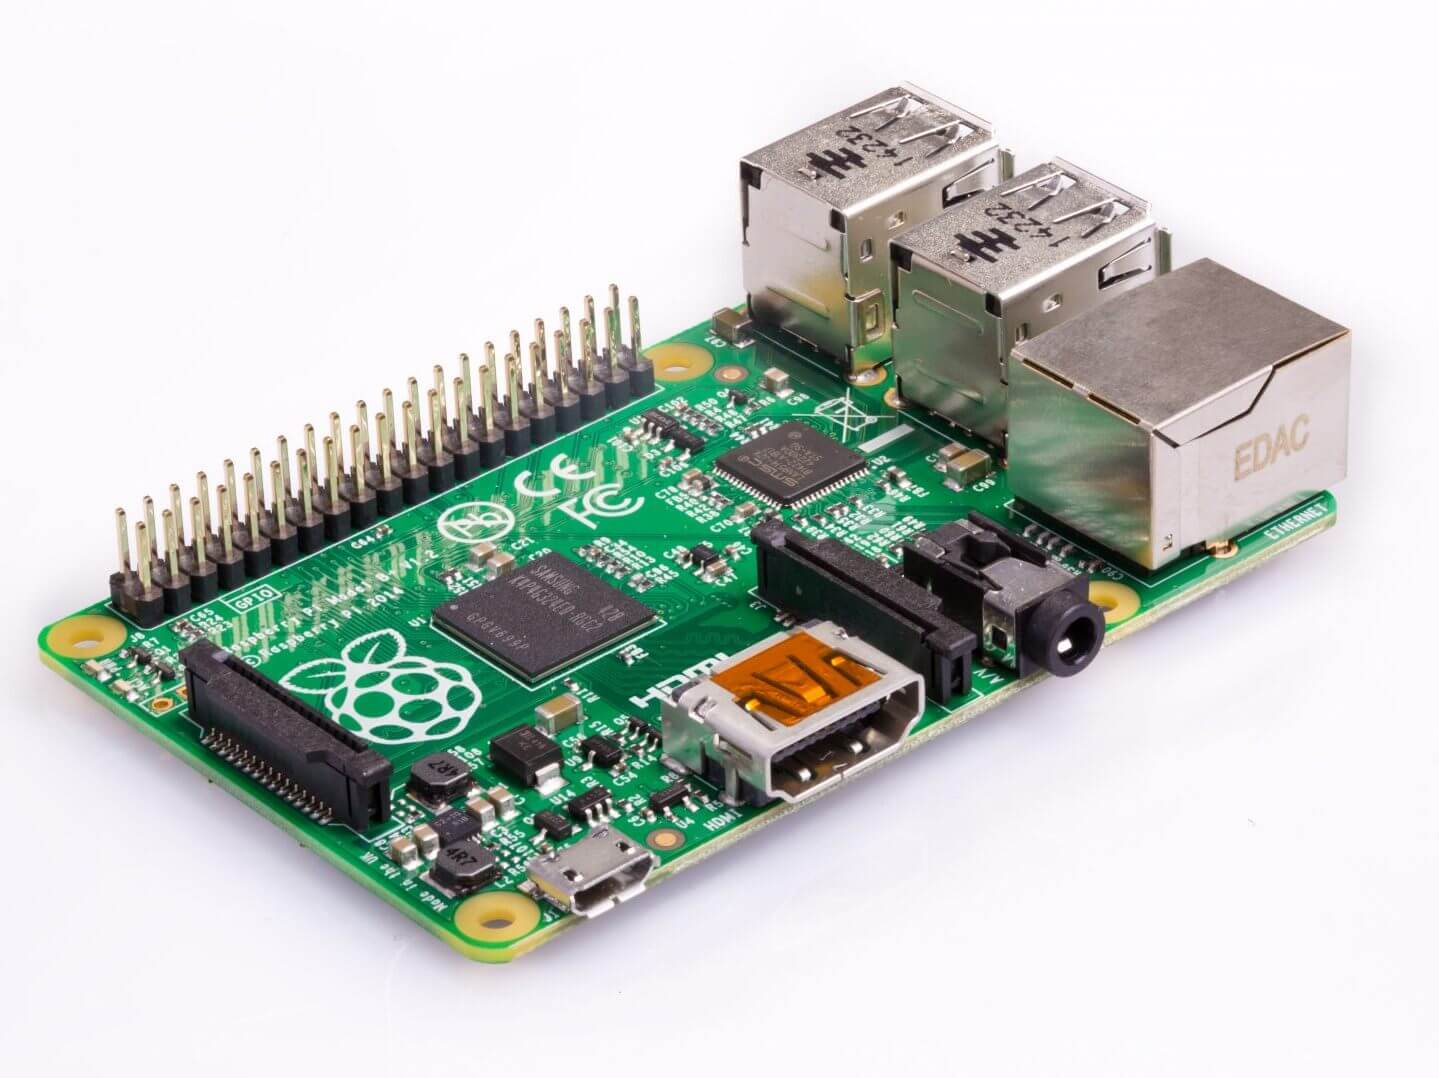
\includegraphics[width=\linewidth]{raspi1B.jpg}
    \end{figure}
\end{columns}

\end{frame}

\begin{frame}{Objectives}
    \textbf{Main goal:}
    to write a configurable operating system for the Raspberry Pi capable on booting on real hardware for educational and hobbyist use. \\~\\

    Specifically, this involves:
    \begin{itemize}
        \item providing different approaches for tasks such as scheduling, interprocess communication, and permanent storage
        \item allowing the user to configure the system at compile time to use different combinations of these approaches, and
        \item exposing a simple and easily extensible interface for additional features
    \end{itemize}
\end{frame}

\begin{frame}{Background material}
    \begin{itemize}
        \item Pintos - Stanford's instructional x86 operating system, used to teach their CS140 course
        \item Baking Pi - Cambridge's tutorial on writing an operating system for the Raspberry Pi in assembly
        \item MINIX - Tanenbaum and Woohull's illustrative operating system for ``Operating Systems: Design and Implementation''
        \item The little book about OS development - Helin and Renberg's ``practical guide to writing your own x86 operating system''
        \item \url{osdev.org/} - community of hobbyist operating system developers, containing information, tutorials, advice, etc.
    \end{itemize}
\end{frame}

\begin{frame}{Why is this project worthwhile?}
\centering
    It is more difficult to get into low-level/systems programming \\
    $\Rightarrow$ focus is on clear code to aid understanding \\~\\

    The project attempts to demystify aspects of operating system development - able to see the theory in practise \\~\\

    It will provide an accessible platform to further tinker and experiment with operating system development, with little to lose
\end{frame}

\begin{frame}{Useful concepts - compilation}
    \textbf{Operating System} - program that manages a computer's hardware \\~\\
    \textbf{Freestanding environment} - little access to C standard library, and program entry point not necessarily at \texttt{main()} \\ $\quad \Rightarrow$ must implement most of standard library ourselves \\~\\
    \textbf{Cross-compiler} - allows us to compile code that will run on the target architecture from our own machine \\~\\
    \textbf{Linker} - responsible for linking all compiled \texttt{.o} files into one executable \\
    Defines the following sections:
    \begin{itemize}
        \item \code{.text} - executable code
        \item \code{.rodata} read-only data (i.e. global constants)
        \item \code{.data} - global variables that are itialised at compile-time
        \item \code{.bss} - uninitialised global variables
    \end{itemize}
\end{frame}

\begin{frame}{Useful concepts - general}
    \textbf{Kernel} - the core of the operating system; the one program which is running at all times throughout execution \\~\\

    \textbf{Exception} - an event triggered when something exceptional happens during normal execution (hardware giving CPU data, privileged action, bad instruction) \\~\\

    \textbf{Process} - a program that has been loaded into memory and is executing \\~\\

    \textbf{Concurrency} - the ability for multiple processes to make progress seemingly simultaneously, as a result of some scheduling algorithm \\~\\

    \textbf{Context Switch} - switching execution to another process. Involves:
    \begin{enumerate}
        \item saving the state of the currently executing process (\textbf{state save})
        \item loading the saved state of a different process (\textbf{state restore})
    \end{enumerate}
\end{frame}

\begin{frame}{Useful concepts - contd.}
    \textbf{Synchronisation} - the prevention of \textbf{race conditions}: when the outcome of two concurrently executing processes depends on the order in which data access took place \\~\\

    \textbf{Interprocess Communication} - mechanism by which cooperating processes may exchange data and information

    \begin{figure}[h]
        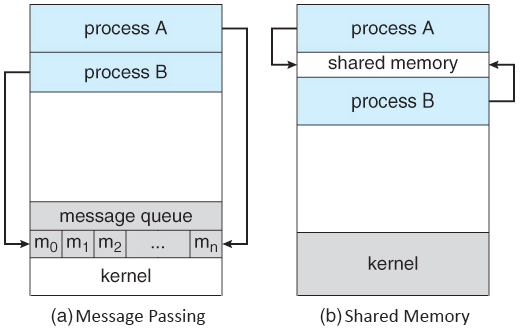
\includegraphics[width=.5\textwidth]{ipc.png}
        \caption{The two fundamental models of interprocess communication}
    \end{figure}

\end{frame}

\begin{frame}{Tools used}
    Languages: C and ARM assembly \\~\\
    Cross-compiler toolchain: \texttt{arm-none-eabi} \\~\\
    Build automation: Make \\~\\
    Version control: git \\~\\
    Emulation: QEMU \\~\\
    Model: Raspberry Pi 1 Model B+
\end{frame}

\begin{frame}{Raspberry Pi 1 Model B+}
    \textbf{Hardware}
    \begin{itemize}
        \item System-on-Chip (SoC): BCM2835
        \item CPU: 700MHz ARM1176JZF-6
        \item GPU: 250MHz Broadcom VideoCore IV
        \item Memory: 512MiB
        \item USB: 4x USB 2.0 ports
        \item Video output: HDMI
        \item Peripherals: 40 GPIO pins, UART
        \item Storage: MicroSD card
    \end{itemize} ~\\

    % or \only
    \onslide<2->{\textbf{Why the Pi in particular?}} \\
    \onslide<3->{Simple boot process - handled entirely by SoC} \\
    \onslide<4->{Underlying architecture of BCM2835 chip is identical to BCM2836/7} \\
    \onslide<5->{Standard set of hardware $\Rightarrow$ more widely accessible}
\end{frame}

\begin{frame}{Project overview}
    Main milestones reached:
    \begin{itemize}
        \item Capable of booting in emulated environment
        \item Capable of booting on real hardware
        \item Display on real screen through HDMI
        \item Interrupts
        \item Processes and Threads
        \item Concurrency
        \item Synchronisation
    \end{itemize} ~\\

    Current goal: interprocess communication
\end{frame}

\begin{frame}[fragile]
    \frametitle{Design overview - boot}
    \textbf{Booting}
    \begin{itemize}
        \item Bootloading handled by SoC, so just need to set up system and initialise C runtime
        \item \texttt{boot.S} initialises stack pointer at \texttt{0x8000}, zeroes \texttt{bss} segment, then loads C kernel entry point \texttt{kernel\_main()} to begin execution
    \end{itemize} ~

    \textbf{Memory management}
    \begin{itemize}
        \item Bootloader creates list of information about the hardware called \textbf{atags}
        \item Each tag consists of a header and tag-specific data
        \item To find the amount of memory available to the system, simply iterate over list of tags until the \texttt{tag == ATAG\_MEM}, at which point return \texttt{atag\_mem.size}
    \end{itemize}

    \begin{columns}[t]
    \column{.6\textwidth}
        \lstset{language=C,basicstyle=\ttfamily}
        \begin{lstlisting}
enum atag_tag {
    ATAG_NONE = 0x00000000,
    ATAG_CORE = 0x54410001,
    ATAG_MEM  = 0x54410002,
    ...
};
        \end{lstlisting}
    \column{.35\textwidth}
        \begin{lstlisting}
struct atag_mem {
    uint32_t size;
    uint32_t start;
};
        \end{lstlisting}
    \end{columns}

\end{frame}

\begin{frame}{Design overview}
    \textbf{Printing to screen}
    \textbf{Interrupts and Exceptions}
    \textbf{System Timer}
    \textbf{Processes and Threads}
    \textbf{Concurrency}
    \textbf{Synchronisation}
    \textbf{Keyboard input}
\end{frame}


\begin{frame}{Project management}

\end{frame}

\begin{frame}{Next steps}

\end{frame}

\begin{frame}{Evaluation}

\end{frame}

\end{document}
